\chapter{Introduction}
\label{cha:introduction}
The aim of this project has been to design and develop Sketchography, an application for users to make a chart of their data by sketching a rough version onto a tablet screen, rather than using a complex Graphical User Interface or programming. The goal is to make an application that's easier for users to pick up than existing charting tools, and one that encourages exploration of the data and various visualisations. I have successfully met all the core requirements, implemented three extensions, and evaluated that the goals were satisfied through a user study.

This chapter documents the motivation for such a project, including previous work in the field, and an overview of what functions the application performs from a user's point of view.

\section{Motivation}
This project is an exploration of Human Computer Interface concepts governing the interactions of users with tools that let them explore and visualise data.

The design of most charting tools is driven by the choice of interface: the mouse and keyboard. Thus, they usually allow graph generation through one of two means:
\begin{enumerate}
\item Configuring a chart template through a number of wizards and dialogue boxes.
\item Manually writing code to generate chart graphics.
\end{enumerate}

Users need to familiarise themselves with how the choices in the wizard, or the commands in the language, translate to graphics.

A better solution is to use a metaphor to a system users have already learnt to use - drawing using pen and paper. Such a system would benefit from matching the users' mental model. 

Additionally, there is a long lag between the users expressing their intention in current systems, and seeing the results of their changes after they close the configuration dialogue or compile and re-run the code. This discourages experimentation and exploration. A better solution would exhibit `liveness' by immediately accommodating users' changes.

\section{Background and Related Work}
Sketching inputs have been studied since the 1960s \citep{sutherland_sketch_1964} as more natural interfaces to computers for graphics-related tasks, compared to indirections like the mouse and keyboard. This has largely been motivated by the widely recognised importance of interactiveness to Information Visualisation (InfoVis) \citep{lee_beyond_2012}. 

Meanwhile, there has been increasing adoption of touch-enabled phones and multi-touch slates amongst the general public, demonstrating people's predilection for what have been referred to as Natural User Interfaces \citep{lee_beyond_2012}. The wide availability of these tools also makes a sketch-based application more feasible to use.


Additionally, \cite{norman_user_1986} describe the `Gulf of Execution', or the gap between a person's intent and their ability to execute that intent. Existing charting tools require users to learn how to accomplish each task, whereas the familiar metaphor of sketching on paper can encourage exploratory work due to the ease of creating changes by visually expressing what sort of change one is trying to make.

There have been a couple of projects that attempt to apply sketch input to the problem domain of creating charts. Microsoft Research's SketchInsight \citep{walny_understanding_2012} lets users make gestures to indicate a type of chart they want. However, by letting the user simply draw the chart they're imagining, rather than making them learn gestures that may not bear a visual resemblance to the end product, Sketchography aims to be easier to learn. Additionally, gestures are immediately converted to charts, which means any further interaction or modifications don't make use of the stylus' digital ink. \cite{chao_poster:_2010} propose a system that lets the user compose basic elements to make visualisations of arbitrary complexity. However, this requires a lot of sketching even for the most basic charts that are commonly used.

In addition to an improved design, this project is also using better sketch recognition techniques, thus reducing the likelihood of frustration due to misclassification of ink strokes.

A larger body of related work is discussed in \autoref{sec:design}, in the context of design decisions made during the implementation of this project.

\section{Project Description}
This paper describes an application that allows the user to sketch a subset of a chart on their computer touch screen as they would on paper. The hypotheses are that, when compared to other charting applications,

\begin{enumerate}
\item[H1] This interface is more `learnable' over time
\item[H2] It encourages exploratory data visualisation creation by making modification easier
\item[H3] Its advantages hold independent of how fluent the user is in English
\end{enumerate}

These hypotheses were investigated through a user study.

The end result is a charting application that works as below:
\begin{enumerate}
\item The user imports data from a Microsoft Excel file.
	\begin{figure}[H]
	\centering
	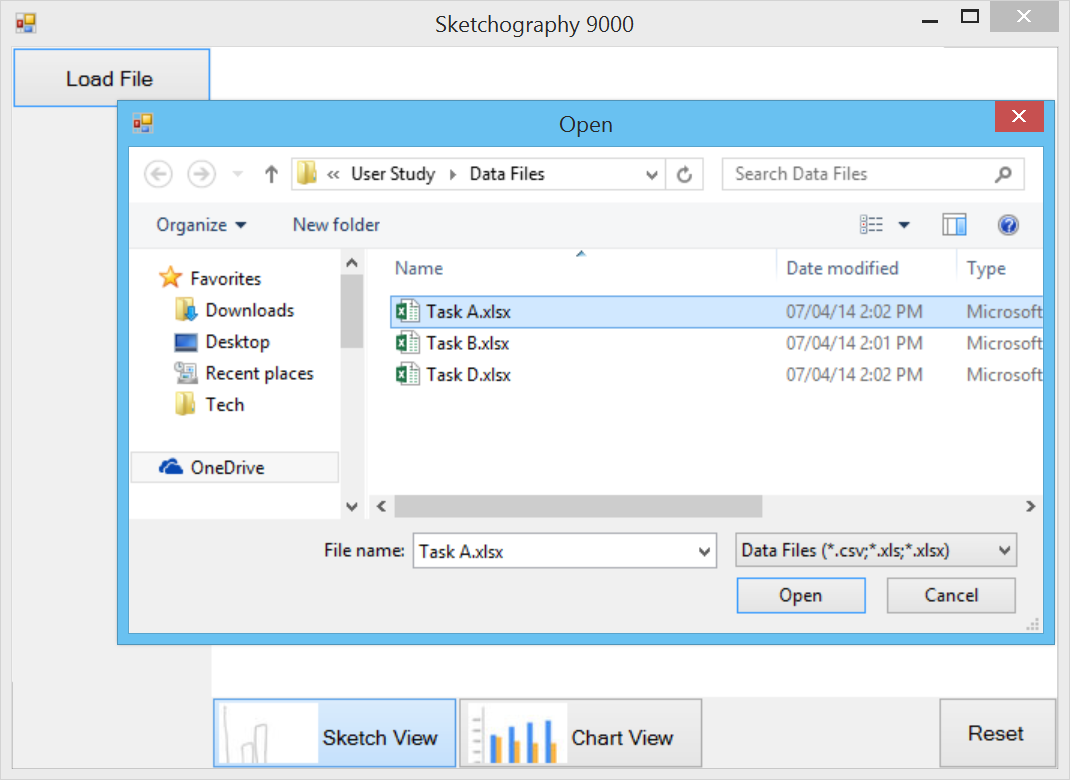
\includegraphics[width=0.6\linewidth]{walk1}
	\end{figure}
\item They sketch a rough indication of a chart.
	\begin{figure}[H]
	\centering
	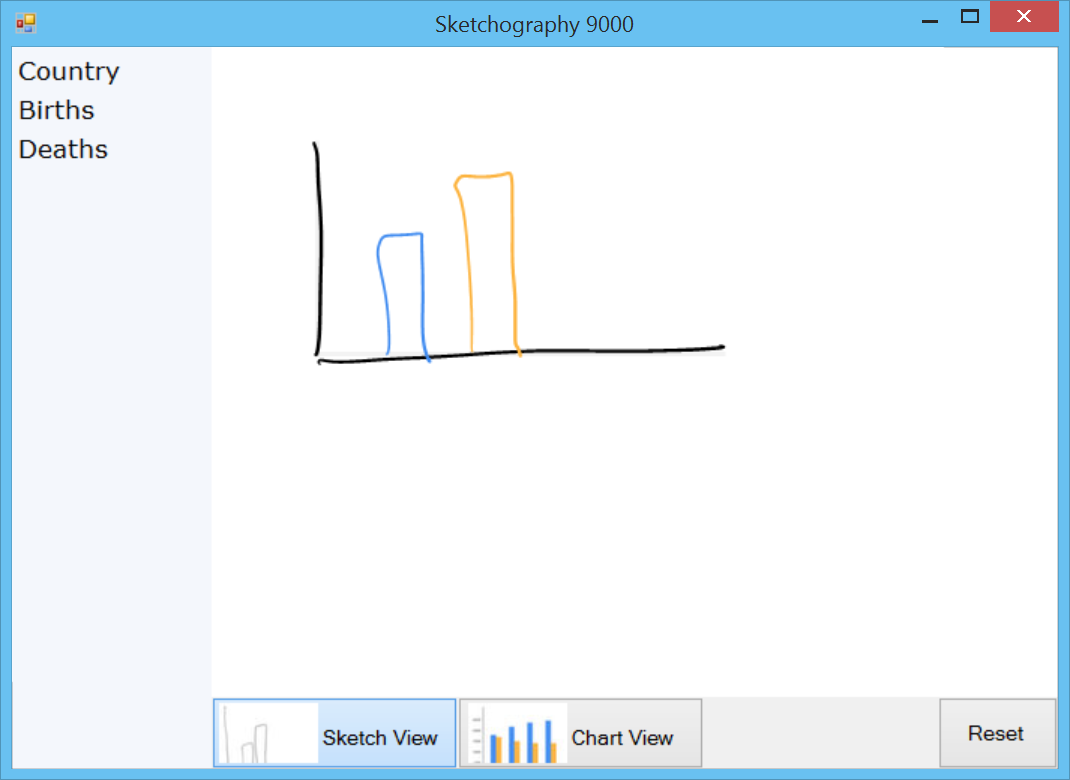
\includegraphics[width=0.6\linewidth]{walk2}
	\end{figure}
\item They drag the data onto elements of the chart to actually bind the data to the chart. 
	\begin{figure}[H]
	\centering
	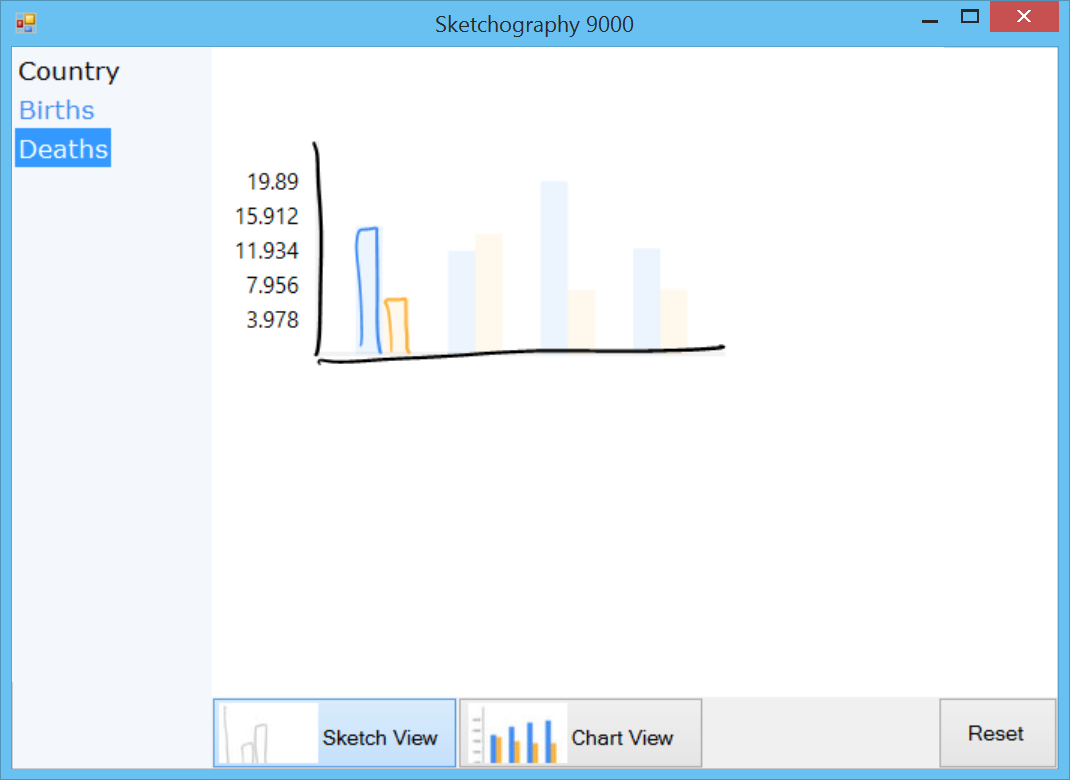
\includegraphics[width=0.6\linewidth]{walk3}
	\end{figure}
\item The tool then creates a 'formal' chart.
	\begin{figure}[H]
	\centering
	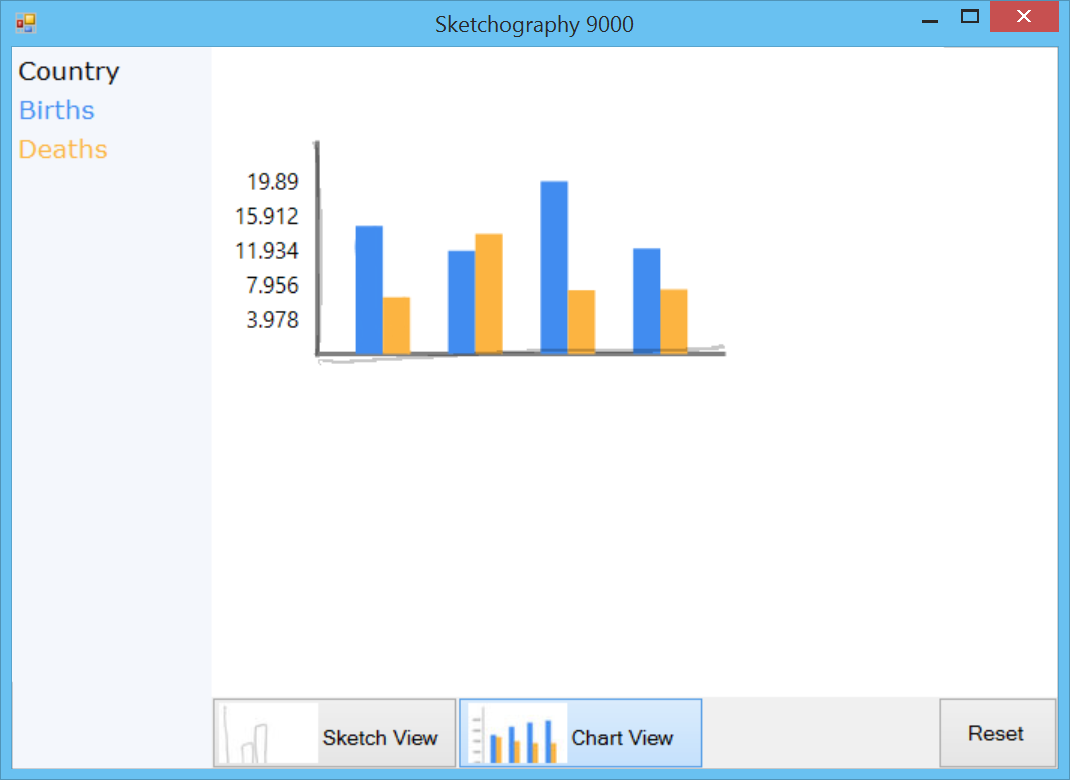
\includegraphics[width=0.6\linewidth]{walk4}
	\end{figure}
\item The tool transforms the user's original sketch to more closely match the formal chart, making the mapping between sketch and formal chart elements evident to the user.
	\begin{figure}[H]
	\centering
	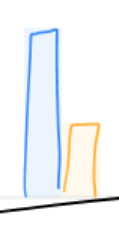
\includegraphics[width=0.1\linewidth]{walk5}
	\end{figure}
\item Any changes on either the sketch or formal chart is fed through to the other view. For example, erasing the a sketched bar removes a data series from the formal bar.
	\begin{figure}[H]
	\centering
	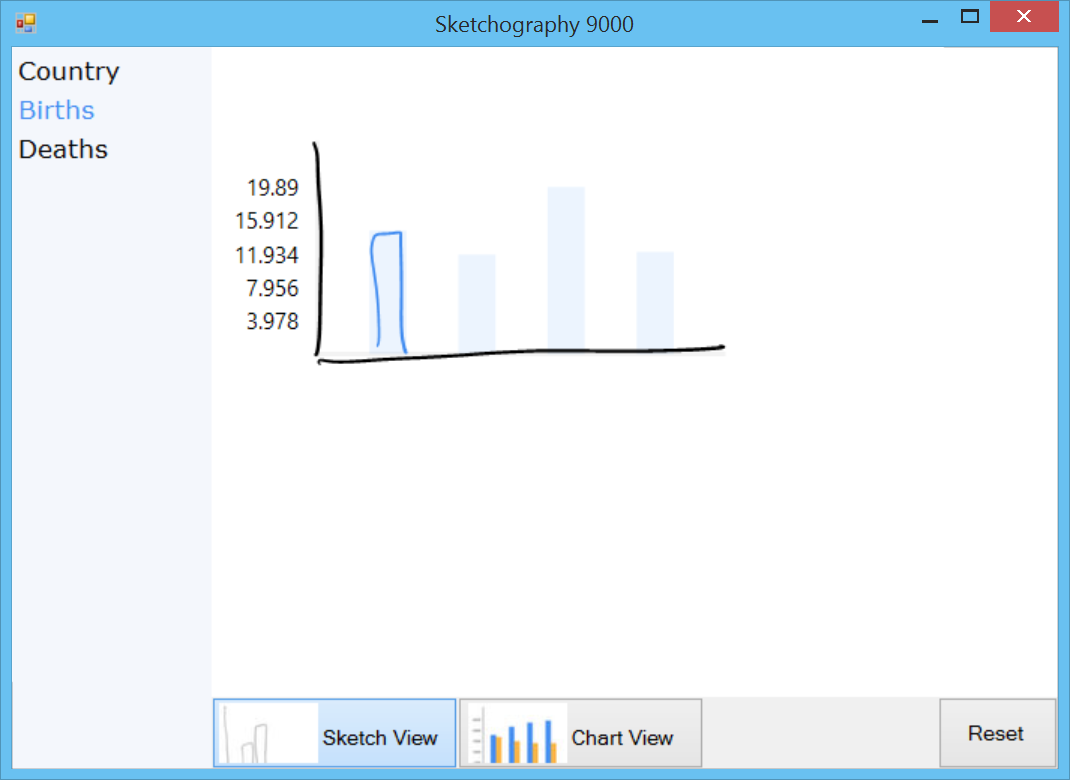
\includegraphics[width=0.6\linewidth]{walk6}
	\end{figure}
\end{enumerate}

\section{Summary}
Existing charting tools are very capable and full-featured, but aren't as easy to learn as they should be, in order to encourage users to explore the data. A new application was proposed that should be easy to learn, and make modifications of the data easy. It uses well-performing data mining algorithms to perform ink stroke recognition, and a charting component to display the data visually. A user study was carried out to confirm that it achieved its goals.
